\documentclass[13pt,compress]{beamer}

\usepackage{../style/lmu-lecture}

\makeatletter
\patchcmd{\beamer@sectionintoc}
  {\vskip0.5\itemsep}
  {}
  {}
\makeatother  

\setbeamertemplate{frametitle}{\expandafter\uppercase\expandafter\insertframetitle}
% remove section slides
\AtBeginSection[]
{
  \begin{frame}[plain]
    \frametitle{\insertsection}
    \tableofcontents[sections={\value{section}}]
  \end{frame}
}

\AtBeginSubsection[]
{
  \begin{frame}<beamer>
    \frametitle{}
\begin{center}    
\LARGE{\subsecname}
\end{center}
  \end{frame}
}
% includepdf slides, pagecommad will set counter for framenumber
\usepackage{pdfpages}
\includepdfset{trim=0mm 0mm 0mm 0mm, pagecommand={\global\setcounter{framenumber}{\value{page}}}}
% add footer:
\usepackage{framed, color}
\usepackage{xcolor}
\setbeamertemplate{footline}[text line]{%
    \noindent\hspace*{\dimexpr-\oddsidemargin-1in\relax}%
     \colorbox{white}{
     \makebox[\dimexpr\paperwidth-2\fboxsep\relax]{
     \color{black}
     \begin{minipage}[c][4.5ex][c]{0.7\linewidth}
       \secname \, | \subsecname
     \end{minipage}
     \hfill\begin{minipage}[c][4.5ex][c]{0.3\linewidth}
       \flushright
       \insertframenumber{}~/~\inserttotalframenumber~~
     \end{minipage}
     }}%
  \hspace*{-\paperwidth}
}

\title{Introduction to Deep Learning}
\author{Prof.~Dr.~David R\"ugamer}
\institute{LMU Munich, MCML}
\date{2024}

\begin{document}
\setbeamercolor{background canvas}{bg=}

% General remark: hyperlinks in included pdfs are not clickable anymore in the combined pdf


\begin{frame}[plain]
  \titlepage
\end{frame}
\begin{frame}[plain]{Contents}
\begin{small}
\tableofcontents[sectionstyle=show/show, subsectionstyle=hide/hide]
\end{small}
\end{frame}
\section{Introduction \& Multilayer Perceptrons}
\subsection{Introduction}
\includepdf[pages={2-last}]{../slides/intro/slides-intro-introduction.pdf}
\subsection{A Brief History}
\includepdf[pages={2-last}]{../slides/intro/slides-intro-brief-history.pdf}
\subsection {A Single Neuron}
\includepdf[pages={2-last}]{../slides/mlps/slides-mlps-single-neuron.pdf}
\subsection {The XOR Problem}
\includepdf[pages={2-last}]{../slides/mlps/slides-mlps-xor.pdf}
\subsection{Single Hidden Layer Networks}
\includepdf[pages={2-last}]{../slides/mlps/slides-mlps-single-hidden-layer-networks.pdf}
\subsection{Multiclass Classification}
\includepdf[pages={2-last}]{../slides/mlps/slides-mlps-multiclass-classification.pdf}
\subsection{Multilayer MLPs}
\includepdf[pages={2-last}]{../slides/mlps/slides-mlps-multilayer-FNNs.pdf}
\subsection{Matrix Notation}

\includepdf[pages={2-last}]{../slides/mlps/slides-mlps-matrix-notation.pdf}
\subsection{Universal Approximation}
\includepdf[pages={2-last}]{../slides/mlps/slides-mlp-univ-approx-theorem.pdf}
\section{Basic Training}
\subsection{Fundamentals}
\includepdf[pages={2-last}]{../slides/opt1/slides-opt1-basic-training.pdf}
\subsection{Computational Graph}
\includepdf[pages={2-last}]{../slides/opt1/slides-opt1-comp-graphs.pdf}
\subsection{Backpropagation}
\includepdf[pages={2-last}]{../slides/opt1/slides-opt1-basic-backpropagation1.pdf}
\includepdf[pages={2-last}]{../slides/opt1/slides-opt1-basic-backpropagation2.pdf}
\subsection{Hardware and Software}
\includepdf[pages={2-last}]{../slides/opt1/slides-opt1-hardware-and-software.pdf}
\section{Regularization}
\subsection{Basic Regularization}
\includepdf[pages={2-last}]{../slides/regu/slides-regu-basic-regularization.pdf}
\subsection{Early Stopping}
\includepdf[pages={2-last}]{../slides/regu/slides-regu-early-stopping.pdf}
\subsection{Dropout and Augmentation}
\includepdf[pages={2-last}]{../slides/regu/slides-regu-ensemble-dropout-augmentation.pdf}
\section{Advanced Optimization}
\subsection{Challenges in Optimization}
\includepdf[pages={2-last}]{../slides/opt2/slides-optim-challenges.pdf}
\subsection{Advanced Optimization}
\includepdf[pages={2-last}]{../slides/opt2/slides-advanced-optim.pdf}
\subsection{Activations}
\includepdf[pages={2-last}]{../slides/opt2/slides-activations.pdf}
\subsection{Initialization}
\includepdf[pages={2-last}]{../slides/opt2/slides-initialization.pdf}
\section{Convolutional Neural Networks}
\subsection{Introduction}
\includepdf[pages={2-last}]{../slides/cnn1/slides-cnn-introduction.pdf} 
\subsection{Conv2D}
\includepdf[pages={2-last}]{../slides/cnn1/slides-cnn-conv2d.pdf} 
\subsection{Properties}
\includepdf[pages={2-last}]{../slides/cnn1/slides-cnn-properties-of-convolution.pdf} 
\subsection{Components}
\includepdf[pages={2-last}]{../slides/cnn1/slides-cnn-components.pdf} 
\subsection{Application}
\includepdf[pages={2-last}]{../slides/cnn1/slides-cnn-application.pdf} 
\subsection{Convolution Types}
\includepdf[pages={2-last}]{../slides/cnn2/slides-convolution-types.pdf} 
\subsection{Dilated and Transposed Convolutions}
\includepdf[pages={2-last}]{../slides/cnn2/slides-dilated-transposed-convolutions.pdf} 
\subsection{Separable and Flattened Convolutions}
\includepdf[pages={2-last}]{../slides/cnn2/slides-separable-convolutions-flattening.pdf} 
\section{Larger CNN Architectures}
\includepdf[pages={2-last}]{../slides/cnn3/slides-modern-cnn-1.pdf} 
\includepdf[pages={2-last}]{../slides/cnn3/slides-modern-cnn-2.pdf} 
\section{Recurrent Networks}
\subsection{Introduction to RNN  and Computational Graph}
\includepdf[pages={2-last}]{../slides/rnn/slides-introduction.pdf} 
\subsection{Backpropagation Through Time}
\includepdf[pages={2-last}]{../slides/rnn/slides-backprop.pdf} 
\subsection{LSTM, GRU, BiRNN}
\includepdf[pages={2-last}]{../slides/rnn/slides-modernrnn.pdf} 
\subsection{RNN Applications}
\includepdf[pages={2-last}]{../slides/rnn/slides-applications.pdf} 
\subsection{Attention Mechanism and Transformers} 
\includepdf[pages={2-last}]{../slides/rnn/slides-attention.pdf} 
\section{Autoencoders}
\subsection{Unsupervised Learning}
\includepdf[pages={2-last}]{../slides/ae/slides-unsupervised-learning.pdf} 
\subsection{Manifold Learning}
\includepdf[pages={2-last}]{../slides/ae/slides-manifold-learning.pdf} 
\subsection{AutoEncoders}
\includepdf[pages={2-last}]{../slides/ae/slides-autoencoders.pdf} 
\subsection{Regularized AE} 
\includepdf[pages={2-last}]{../slides/ae/slides-autoencoders-regularized.pdf} 
\subsection{Specific AE} 
\includepdf[pages={2-last}]{../slides/ae/slides-autoencoders-specific.pdf} 
\subsection{Variational AE}
\includepdf[pages={2-last}]{../slides/ae/slides-vae.pdf} 
\section{Generative Adversarial Networks}
\subsection{Generative Models}
\includepdf[pages={2-last}]{../slides/generative_models/slides-introduction.pdf} 
\subsection{Introduction GANs}
\includepdf[pages={2-last}]{../slides/generative_models/slides-GAN-intro.pdf} 
\subsection{Variants}
\includepdf[pages={2-last}]{../slides/generative_models/slides-GAN-variants.pdf} 
\subsection{Challenges}
\includepdf[pages={2-last}]{../slides/generative_models/slides-GAN-challenges.pdf} 
\section{Adversarial Examples}
\includepdf[pages={2-last}]{../slides/adversarial_attacks/slides-adversarials.pdf} 

\end{document}
